\documentclass[a4paper, oneside]{discothesis}

\usepackage[utf8]{inputenc}
\usepackage[T1]{fontenc}
\usepackage{algpseudocode}
\usepackage{algorithm}
\usepackage{mathtools}
\usepackage{subcaption}
\usepackage{tikz}
\usetikzlibrary{arrows.meta}


%%%%%%%%%%%%%%%%%%%%%%%%%%%%%%%%%%%%%%%%%%%%%%%%%%%%%%%%%%%%%%%%%%%%%%%%%%%%%%%%%%%%%%%%%%%%%%%%%
% DOCUMENT METADATA

\thesistype{Bachelor's Thesis} % Master's Thesis, Bachelor's Thesis, Semester Thesis, Group Project
\title{Practical Dynamic Directories}

\author{Silvan Mosberger}
\email{msilvan@student.ethz.ch}

\institute{Distributed Computing Group \\[2pt]
Computer Engineering and Networks Laboratory \\[2pt]
ETH Zürich}

\supervisors{András Papp, Pankaj Khanchandani\\[2pt] Prof.\ Dr.\ Roger Wattenhofer}

% Optionally, keywords and categories of the work can be shown (on the Abstract page)
\keywords{Arrow, Ivy, distributed directory, shared object}
\categories{Network algorithms}

\date{\today}

%%%%%%%%%%%%%%%%%%%%%%%%%%%%%%%%%%%%%%%%%%%%%%%%%%%%%%%%%%%%%%%%%%%%%%%%%%%%%%%%%%%%%%%%%%%%%%%%%

\begin{document}

\frontmatter % do not remove this line
\maketitle

\cleardoublepage

\begin{acknowledgements}
I thank Lorem ipsum dolor sit amet, consetetur sadipscing elitr, sed diam nonumy eirmod tempor invidunt ut labore et dolore magna aliquyam erat, sed diam voluptua. At vero eos et accusam et justo duo dolores et ea rebum. Stet clita kasd gubergren, no sea takimata sanctus est Lorem ipsum dolor sit amet. Lorem ipsum dolor sit amet, consetetur sadipscing elitr, sed diam nonumy eirmod tempor invidunt ut labore et dolore magna aliquyam erat, sed diam voluptua. At vero eos et accusam et justo duo dolores et ea rebum. Stet clita kasd gubergren, no sea takimata sanctus est Lorem ipsum dolor sit amet.
\end{acknowledgements}


\begin{abstract}
The abstract should be short, stating what you did and what the most important result is.
Lorem ipsum dolor sit amet, consetetur sadipscing elitr, sed diam nonumy eirmod tempor invidunt ut labore et dolore magna aliquyam erat, sed diam voluptua. At vero eos et accusam et justo duo dolores et ea rebum. Stet clita kasd gubergren, no sea takimata sanctus est Lorem ipsum dolor sit amet. Lorem ipsum dolor sit amet, consetetur sadipscing elitr, sed diam nonumy eirmod tempor invidunt ut labore et dolore magna aliquyam erat, sed diam voluptua. At vero eos et accusam et justo duo dolores et ea rebum. Stet clita kasd gubergren, no sea takimata sanctus est Lorem ipsum dolor sit amet.
\end{abstract}

\tableofcontents

\mainmatter

\chapter{Introduction}

Should include
\begin{itemize}
\item Explanation of what problem such algs solve
\item Explanation of the model used, nodes know local weights
\item Explain Arvy, Arrow and Ivy, with pictures if possible
\end{itemize}

Often in computing a single resource is shared between multiple components, where only one of them may access it at a time. In a distributed setting an algorithm to solve this is called a distributed mutual exclusion algorithm or distributed directory protocol. A trivial solution is to dedicate a single node to be the center where all requests for the resource should go, with the disadvantage of a lot of traffic for many requests. Better solutions to this problem include the Arrow and Ivy protocols, both of which work on similar principles to be explained in the following sections. In the Arvy paper these protocols have been combined in a flexible manner to allow a whole set of algorithms to be created.

In this thesis we explore this set of Arvy algorithms in the hopes of finding ones that work better than any already existing ones.

\section{Model}

We consider a complete graph $G=(V,E)$ with $n\coloneqq|V|$ vertices and $m\coloneqq\binom{n}{2}$ edges. Each edge has a cost $c : E \rightarrow \mathbb{R}$ associated with it, representing the amount of time it takes a message to traverse it. The costs form a metric space:
\begin{itemize}
\item The cost from a node to itself is zero: $\forall v:c(v, v)=0$
\item Costs between different nodes are positive: $\forall u,v : u\neq v\Rightarrow c(u,v)>0$
\item Costs are the same in both directions: $\forall u,v : c(u,v)=c(v,u)$
\item Triangle inequality: $\forall u,v,w : c(u,w)\leq c(u,v)+c(v,w)$
\end{itemize}

As a reasonable constraint, a node $v$ can only query costs from itself to other nodes, so it has access to $\{c(v, u)\;|\;u\in V\}$. In a realistic scenario these costs can be obtained and updated by doing regular pings to other nodes. In our model we don't consider changing costs however.

As a major simplification, nodes only request the token in series. So only after the token has reached the requesting node another node can make a request for it. Therefore requests can be represented as an infinite series $r=\{r_i\},i\in\mathbb{N},r_i\in N$ where $r_i$ encodes the $i$-th request originating from node $r_i$.

\section{Arrow, Ivy and Arvy}

In this section we explain how Arrow, Ivy and Arvy work. Because Arvy is a generalization of both Arrow and Ivy, we start with it and specialize it to the others later.

\subsection{Arvy}

Arvy is based on the idea of maintaining a rooted spanning tree over time: Every node stores a pointer to its parent $parent : V \rightarrow V$ while root nodes point to themselves. When a (non-root) node $a_0$ needs the token, it sends a request message towards its parent $a_1=parent(a_0)$. When a node $a_i$ receives such a request, it forwards it to $a_{i+1}=parent(a_i)$ and so on until the root $a_k$ containing the token is reached. This forms a request path $\{a_0,a_1,\dots,a_k\}$ of $k-1$ nodes. The final node then finishes its own work with the token after which it sends it directly to $a_0$. The interesting idea with Arvy is that each node $a_i$ receiving the request updates its parent to a node in $\{a_0, \dots, a_{i-1}\}$, so one of the nodes the request previously visited.

It's easy to see that this algorithm maintains a spanning tree over time with sequential requests. However this also holds for concurrent requests as the Arvy paper~\cite{Arvy} shows. Perhaps by surprise this means that no matter what the \textsc{SelectNewParent} function returns out of the given arguments, it can't prevent the algorithm from being correct.

\begin{algorithm}
\caption{Arvy algorithm}
\label{test}
\begin{algorithmic}

\Function{RequestToken}{$a_0$}
\If{$parent(a_0)\neq a_0$}
    \State send request for token to $parent(a_0)$
    \State $parent(a_0)\gets a_0$
\EndIf
\EndFunction
\Function{ReceiveRequest}{$a_k$}
\If{$parent(a_k)=a_k$}
    \State send token to $a_0$
\Else
    \State forward request to $parent(a_k)$
\EndIf
\State $parent(a_k)\gets\;$\Call{SelectNewParent}{$a_0, a_1, \dots, a_{k-1}$}
\EndFunction
\Function{SelectNewParent}{$\{a_i\}$}
\State\Return any of $a_i$
\EndFunction
\end{algorithmic}
\end{algorithm}

\begin{figure}[]
\begin{subfigure}[t]{0.5\textwidth}
\centering
\begin{tikzpicture}
[bn/.style={circle,draw}
,root/.style={bn,thick}
,be/.style={draw=black,arrows={-Stealth[scale=1.5]}}
,req/.style={bn,red!70!black}
,auto,scale=0.7]
\node[root] (n1) at (0,5) {1};
\node[req] (n2) at (7,5) {2};
\node[above=0 of n2, red!70!black] {needs token};
\node[bn] (n3) at (3,4) {3};
\node[bn] (n4) at (2,1) {4};
\node[bn] (n5) at (6,0) {5};
\draw[be] (n2) -- (n3);
\draw[be] (n4) -- (n3);
\draw[be] (n5) -- (n4);
\draw[be] (n3) -- (n1);
\end{tikzpicture}
\caption{Node 2 needs the token}
\end{subfigure}
\quad
\begin{subfigure}[t]{0.5\textwidth}
\centering
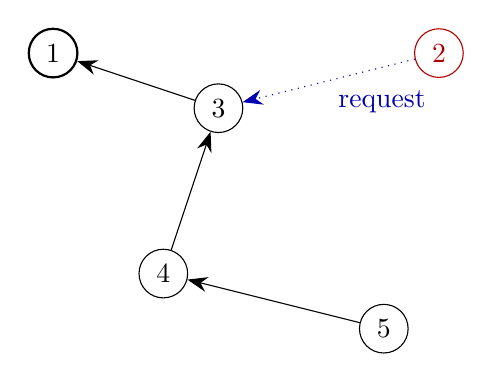
\begin{tikzpicture}
[bn/.style={circle,draw}
,root/.style={bn,thick}
,be/.style={draw=black,arrows={-Stealth[scale=1.5]}}
,req/.style={bn,red!70!black}
,auto,scale=0.7]
\node[root] (n1) at (0,5) {1};
\node[req] (n2) at (7,5) {2};
\node[bn] (n3) at (3,4) {3};
\node[bn] (n4) at (2,1) {4};
\node[bn] (n5) at (6,0) {5};
\draw[be] (n4) -- (n3);
\draw[be] (n5) -- (n4);
\draw[be] (n3) -- (n1);
\draw[be,dotted,blue!70!black] (n2) -- node{request} (n3);
\end{tikzpicture}
\caption{Node 2 sends a request towards its parent after which it sets its parent to itself}
\end{subfigure}

\begin{subfigure}[t]{0.5\textwidth}
\centering
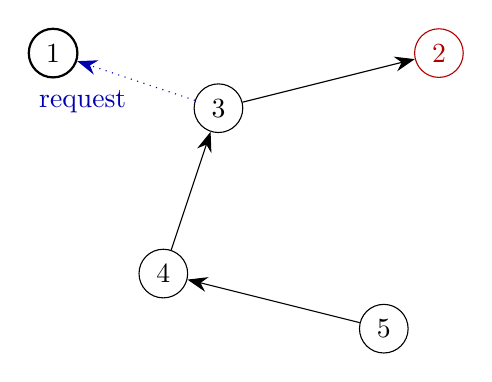
\begin{tikzpicture}
[bn/.style={circle,draw}
,root/.style={bn,thick}
,be/.style={draw=black,arrows={-Stealth[scale=1.5]}}
,req/.style={bn,red!70!black}
,auto,scale=0.7]
\node[root] (n1) at (0,5) {1};
\node[req] (n2) at (7,5) {2};
\node[bn] (n3) at (3,4) {3};
\node[bn] (n4) at (2,1) {4};
\node[bn] (n5) at (6,0) {5};
\draw[be] (n4) -- (n3);
\draw[be] (n5) -- (n4);
\draw[be] (n3) -- (n2);
\draw[be,dotted,blue!70!black] (n3) -- node{request} (n1);
\end{tikzpicture}
\caption{Node 3 receives the request and forwards it to its parent while changing its parent to the only previously visited node 2}
\end{subfigure}
\quad
\begin{subfigure}[t]{0.5\textwidth}
\centering
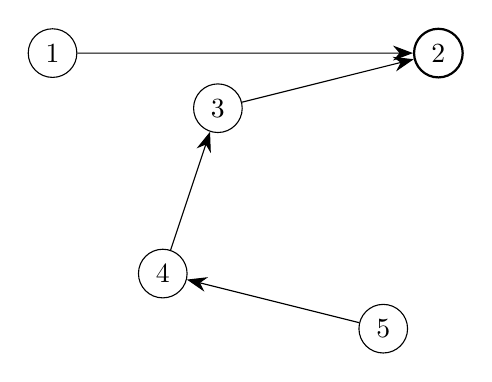
\begin{tikzpicture}
[bn/.style={circle,draw}
,root/.style={bn,thick}
,be/.style={draw=black,arrows={-Stealth[scale=1.5]}}
,req/.style={bn,red!70!black}
,auto,scale=0.7]
\node[bn] (n1) at (0,5) {1};
\node[root] (n2) at (7,5) {2};
\node[bn] (n3) at (3,4) {3};
\node[bn] (n4) at (2,1) {4};
\node[bn] (n5) at (6,0) {5};
\draw[be] (n4) -- (n3);
\draw[be] (n5) -- (n4);
\draw[be] (n3) -- (n2);
\draw[be] (n1) -- (n2);
\end{tikzpicture}
\caption{Node 1 which has the token receives the request, it sends the token to 2, making it the new root. Out of the possible new parents $\{2,3\}$ it chooses 2}
\end{subfigure}

\begin{subfigure}[t]{0.5\textwidth}
\centering
\begin{tikzpicture}
[bn/.style={circle,draw}
,root/.style={bn,thick}
,be/.style={draw=black,arrows={-Stealth[scale=1.5]}}
,req/.style={bn,red!70!black}
,auto,scale=0.7]
\node[bn] (n1) at (0,5) {1};
\node[root] (n2) at (7,5) {2};
\node[bn] (n3) at (3,4) {3};
\node[bn] (n4) at (2,1) {4};
\node[req] (n5) at (6,0) {5};
\node[above=0 of n5, red!70!black] {needs token};
\draw[be] (n4) -- (n3);
\draw[be] (n5) -- (n4);
\draw[be] (n3) -- (n2);
\draw[be] (n1) -- (n2);
\draw[be,dotted,blue!70!black] (n5) .. controls (n4) and (n3) .. node[right]{request} (n2);
\end{tikzpicture}
\caption{Node 5 needs the token, resulting in a request path over $\{5,4,3,2\}$}
\end{subfigure}
\quad
\begin{subfigure}[t]{0.5\textwidth}
\centering
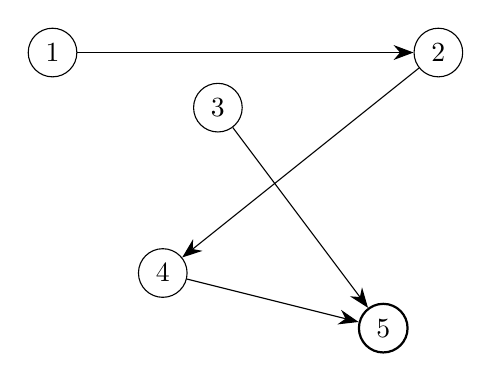
\begin{tikzpicture}
[bn/.style={circle,draw}
,root/.style={bn,thick}
,be/.style={draw=black,arrows={-Stealth[scale=1.5]}}
,req/.style={bn,red!70!black}
,auto,scale=0.7]
\node[bn] (n1) at (0,5) {1};
\node[bn] (n2) at (7,5) {2};
\node[bn] (n3) at (3,4) {3};
\node[bn] (n4) at (2,1) {4};
\node[root] (n5) at (6,0) {5};
\draw[be] (n2) -- (n4);
\draw[be] (n4) -- (n5);
\draw[be] (n3) -- (n5);
\draw[be] (n1) -- (n2);
\end{tikzpicture}
\caption{After node 2 with the token received the request it sent it to node 5. The nodes 4, 3 and 2 on the request path were able to choose its new parent from $\{5\}$, $\{5,4\}$ and $\{5,4,3\}$ respectively.}
\end{subfigure}
\caption{Arvy example}
\end{figure}

\subsection{Arrow}

Arrow is a specialized version of Arvy that makes nodes along the request path always select the most recent node as a new parent
\begin{algorithmic}
\Function{SelectNewParent}{$\{a_i\}$}
\State\Return $a_i$
\EndFunction
\end{algorithmic}

\subsection{Ivy}

Similarly, Ivy is a specialized version of Arvy that makes nodes along the request path always select the oldest node as a new parent, which is always the node that made the request originally
\begin{algorithmic}
\Function{SelectNewParent}{$\{a_i\}$}
\State\Return $a_0$
\EndFunction
\end{algorithmic}

\chapter{Test data}

Should include
\begin{itemize}
\item Explanation of all algorithms, initial trees, weights and requests to be used
\end{itemize}

\chapter{Results}

Should include
\begin{itemize}
\item Resulting plots of interesting evaluations
\item Show how to reproduce the results including parameters
\end{itemize}

\chapter{Program Design}

Should include
\begin{itemize}
\item How the program design only allows expressing valid Arvy algorithms
\end{itemize}


\begin{theorem}[First Theorem]\label{thm:first theorem}
	This is our first theorem.
\end{theorem}

\begin{proof}
	And this is the proof of the first theorem with a complicated formula and a reference to Theorem \ref{thm:first theorem}. Lorem ipsum dolor sit amet, consetetur sadipscing elitr, sed diam nonumy eirmod tempor invidunt ut labore et dolore magna aliquyam erat, sed diam voluptua. Lorem ipsum dolor sit amet, consetetur sadipscing elitr, sed diam nonumy eirmod tempor invidunt ut labore et dolore magna aliquyam erat, sed diam voluptua.
	\begin{equation}
		{\frac {\mathrm d}{\mathrm dx}}\arctan(\sin({x}^{2}))=-2 \cdot {\frac {\cos({x}^{2})x}{-2+\left (\cos({x}^{2})\right )^{2}}}
	\end{equation}	
\end{proof}

\begin{figure}
    \centering
    \includegraphics[width=0.2\columnwidth]{figures/disco_logo_faded}
    \caption{This is an example graphic.}
    \label{fig:example_figure}
\end{figure}

And here we cite some external documents~\cite{TestReference, TestReference2}.
An example of an included graphic can be found in Figure~\ref{fig:example_figure}.
Note that in \LaTeX, ``quotes'' do not use the usual double quote characters.

% This displays the bibliography for all cited external documents. All references have to be defined in the file references.bib and can then be cited from within this document.
\bibliographystyle{IEEEtran}
\bibliography{references}

% This creates an appendix chapter, comment if not needed.
\appendix
\chapter{First Appendix Chapter Title}

\end{document}
